\documentclass[11pt,a4paper]{report}
\usepackage[textwidth=37em,vmargin=30mm]{geometry}
\usepackage{calc,xunicode,amsmath,amssymb,paralist,enumitem,tabu,booktabs,datetime2,xeCJK,xeCJKfntef,listings}
\usepackage{tocloft,fancyhdr,tcolorbox,xcolor,graphicx,eso-pic,xltxtra,xelatexemoji}

\newcommand{\envyear}[0]{2024}
\newcommand{\envdatestr}[0]{2024-10-16}
\newcommand{\envfinaldir}[0]{webdb/2024/20241016/final}

\usepackage[hidelinks]{hyperref}
\hypersetup{
    colorlinks=false,
    pdfpagemode=FullScreen,
    pdftitle={Web Digest - \envdatestr}
}

\setlength{\cftbeforechapskip}{10pt}
\renewcommand{\cftchapfont}{\rmfamily\bfseries\large\raggedright}
\setlength{\cftbeforesecskip}{2pt}
\renewcommand{\cftsecfont}{\sffamily\small\raggedright}

\setdefaultleftmargin{2em}{2em}{1em}{1em}{1em}{1em}

\usepackage{xeCJK,xeCJKfntef}
\xeCJKsetup{PunctStyle=plain,RubberPunctSkip=false,CJKglue=\strut\hskip 0pt plus 0.1em minus 0.05em,CJKecglue=\strut\hskip 0.22em plus 0.2em}
\XeTeXlinebreaklocale "zh"
\XeTeXlinebreakskip = 0pt


\setmainfont{Brygada 1918}
\setromanfont{Brygada 1918}
\setsansfont{IBM Plex Sans}
\setmonofont{JetBrains Mono NL}
\setCJKmainfont{Noto Serif CJK SC}
\setCJKromanfont{Noto Serif CJK SC}
\setCJKsansfont{Noto Sans CJK SC}
\setCJKmonofont{Noto Sans CJK SC}

\setlength{\parindent}{0pt}
\setlength{\parskip}{8pt}
\linespread{1.15}

\lstset{
	basicstyle=\ttfamily\footnotesize,
	numbersep=5pt,
	backgroundcolor=\color{black!5},
	showspaces=false,
	showstringspaces=false,
	showtabs=false,
	tabsize=2,
	captionpos=b,
	breaklines=true,
	breakatwhitespace=true,
	breakautoindent=true,
	linewidth=\textwidth
}






\newcommand{\coverpic}[2]{
    % argv: itemurl, authorname
    Cover photo by #2~~(\href{#1}{#1})
}
\newcommand{\makeheader}[0]{
    \begin{titlepage}
        % \newgeometry{hmargin=15mm,tmargin=21mm,bmargin=12mm}
        \begin{center}
            
            \rmfamily\scshape
            \fontspec{BaskervilleF}
            \fontspec{Old Standard}
            \fontsize{59pt}{70pt}\selectfont
            WEB\hfill DIGEST
            
            \vfill
            % \vskip 30pt
            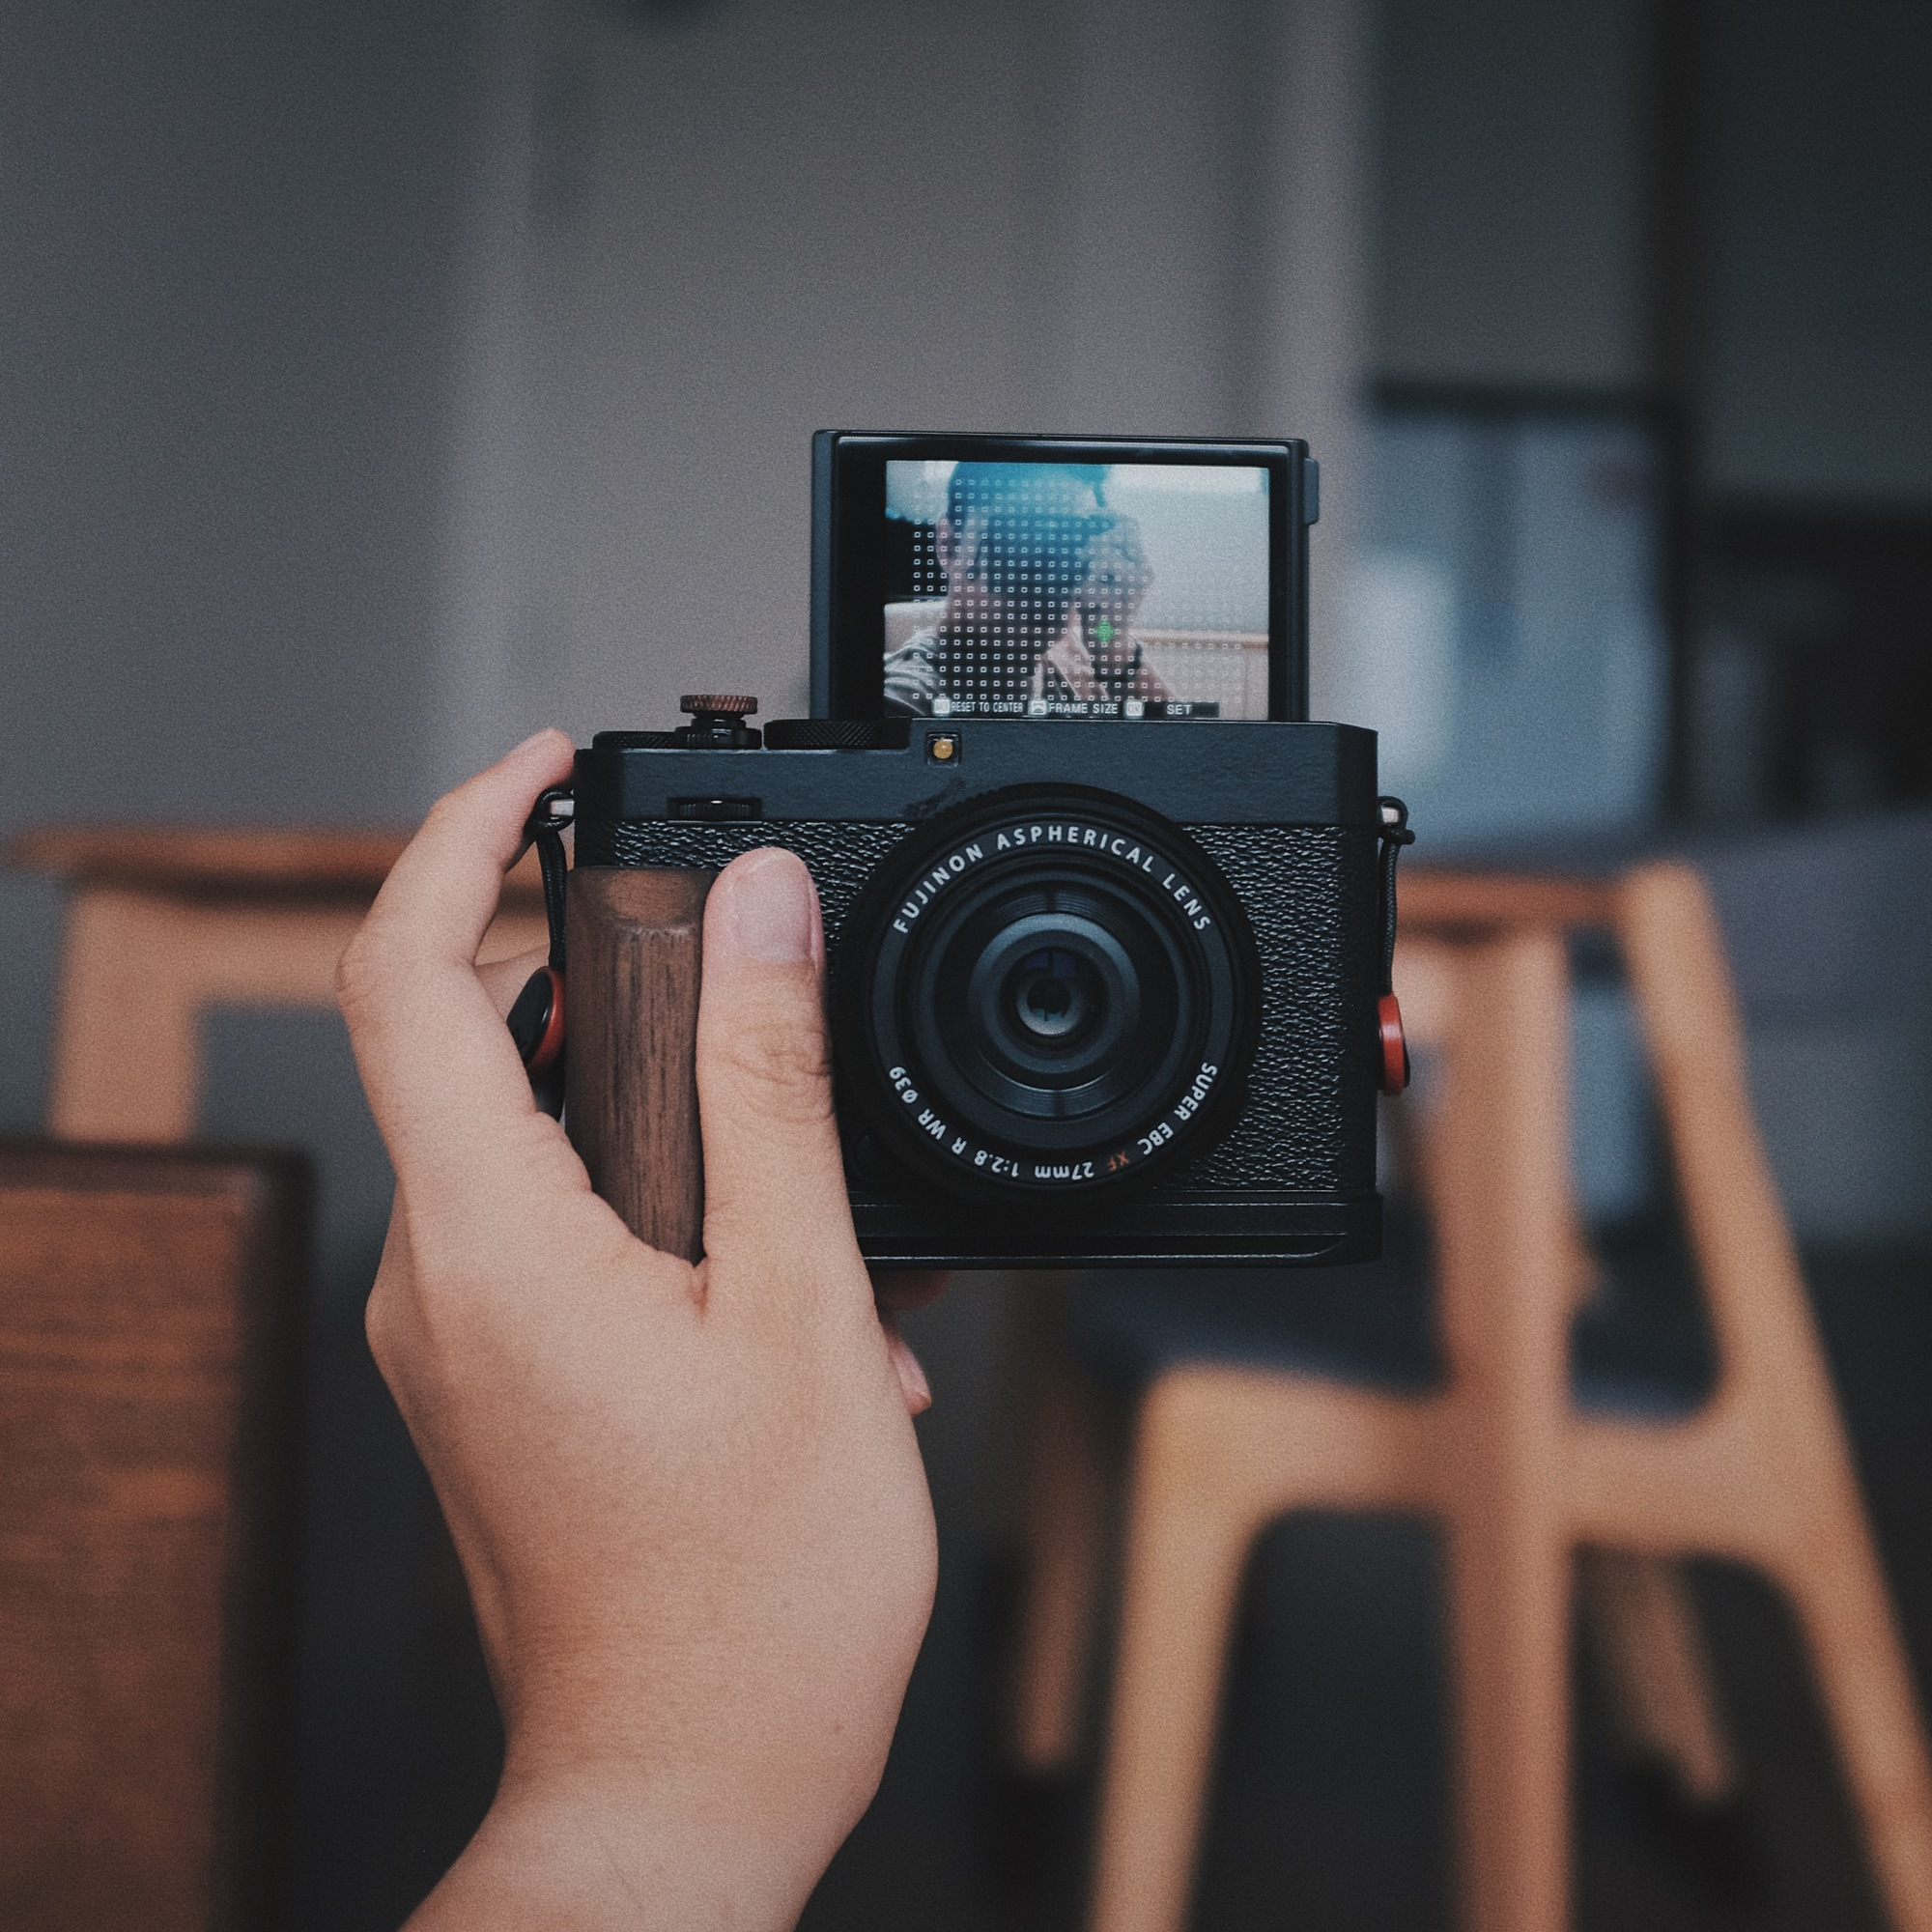
\includegraphics[width=\linewidth]{\envfinaldir/coverpic-prod.jpg}\par
            % \vskip 30pt
            \vfill

            \normalsize\rmfamily\scshape
            \copyright{} The Web Digest Project \hfill\large \envdatestr
        \end{center}
    \end{titlepage}
    % \restoregeometry
}
\newcommand{\simplehref}[1]{%
    \textcolor{blue!80!green}{\href{#1}{#1}}%
}
\renewcommand{\contentsname}{\center\Huge\sffamily\bfseries Contents\par\vskip 20pt}
\newcounter{ipartcounter}
\setcounter{ipartcounter}{0}
\newcommand{\ipart}[1]{
    % \vskip 20pt
    \clearpage
    \stepcounter{ipartcounter}
    \phantomsection
    \addcontentsline{toc}{chapter}{#1}
    % \begin{center}
    %     \Huge
    %     \sffamily\bfseries
    %     #1
    % \end{center}
    % \vskip 20pt plus 7pt
}
\newcounter{ichaptercounter}
\setcounter{ichaptercounter}{0}
\newcommand{\ichapter}[1]{
    % \vskip 20pt
    \clearpage
    \stepcounter{ichaptercounter}
    \phantomsection
    \addcontentsline{toc}{section}{\numberline{\arabic{ichaptercounter}}#1}
    \begin{center}
        \Huge
        \sffamily\bfseries
        #1
    \end{center}
    \vskip 20pt plus 7pt
}
\newcommand{\entrytitlefont}[1]{\subsection*{\raggedright\Large\sffamily\bfseries#1}}
\newcommand{\entryitemGeneric}[2]{
    % argv: title, url
    \parbox{\linewidth}{
        \entrytitlefont{#1}\par\vskip 5pt
        \footnotesize\ttfamily\mdseries
        \simplehref{#2}
    }\vskip 11pt plus 11pt minus 1pt
}
\newcommand{\entryitemGithub}[3]{
    % argv: title, url, desc
    \parbox{\linewidth}{
        \entrytitlefont{#1}\par\vskip 5pt
        \footnotesize\ttfamily\mdseries
        \simplehref{#2}\par\vskip 5pt
        \small\rmfamily\mdseries#3
    }\vskip 11pt plus 11pt minus 1pt
}
\newcommand{\entryitemAp}[3]{
    % argv: title, url, desc
    \parbox{\linewidth}{
        \entrytitlefont{#1}\par\vskip 5pt
        \footnotesize\ttfamily\mdseries
        \simplehref{#2}\par\vskip 5pt
        \small\rmfamily\mdseries#3
    }\vskip 11pt plus 11pt minus 1pt
}
\newcommand{\entryitemHackernews}[3]{
    % argv: title, hnurl, rawurl
    % \parbox{\linewidth}{
    %     \entrytitlefont{#1}\par\vskip 5pt
    %     \footnotesize\ttfamily\mdseries
    %     \simplehref{#3}\par
    %     \textcolor{black!50}{\href{#2}{#2}}
    % }\vskip 11pt plus 11pt minus 1pt
    \begin{minipage}{\linewidth}
            \entrytitlefont{#1}\par\vskip 5pt
            \footnotesize\ttfamily\mdseries
            \simplehref{#3}\par
            \textcolor{black!50}{\href{#2}{#2}}
    \end{minipage}\par\vskip 11pt plus 11pt minus 1pt
}







\begin{document}

\makeheader

\tableofcontents\clearpage




\ipart{Developers}
\ichapter{Hacker News}
\entryitemTwoLinks{Sqlite3 WebAssembly}{https://news.ycombinator.com/item?id=41851051}{https://sqlite.org/wasm/doc/trunk/index.md}

\entryitemTwoLinks{The C23 edition of Modern C}{https://news.ycombinator.com/item?id=41850017}{https://gustedt.wordpress.com/2024/10/15/the-c23-edition-of-modern-c/}

\entryitemTwoLinks{OpenAI Is a Bad Business}{https://news.ycombinator.com/item?id=41849735}{https://www.wheresyoured.at/oai-business/}

\entryitemTwoLinks{Apple introduces iPad mini built for Apple Intelligence}{https://news.ycombinator.com/item?id=41849058}{https://www.apple.com/newsroom/2024/10/apple-introduces-powerful-new-ipad-mini-built-for-apple-intelligence/}

\entryitemTwoLinks{Life expectancy rise in rich countries slows down: took 30 years to prove}{https://news.ycombinator.com/item?id=41848482}{https://www.nature.com/articles/d41586-024-03244-1}

\entryitemTwoLinks{Show HN: I built the most over-engineered Deal With It emoji generator}{https://news.ycombinator.com/item?id=41848150}{https://emoji.build/deal-with-it-generator/}

\entryitemTwoLinks{Web Browser Engineering (2021)}{https://news.ycombinator.com/item?id=41846780}{https://browser.engineering/index.html}

\entryitemTwoLinks{Show HN: Pumpkin – A Modern Minecraft server written in Rust}{https://news.ycombinator.com/item?id=41846636}{https://github.com/Snowiiii/Pumpkin}

\entryitemTwoLinks{SSL certificate lifetimes are going down. Dates proposed. 45 days by 2027}{https://news.ycombinator.com/item?id=41845885}{https://github.com/cabforum/servercert/pull/553}

\entryitemTwoLinks{The American economy has left other rich countries in the dust}{https://news.ycombinator.com/item?id=41845705}{https://www.economist.com/special-report/2024/10/14/the-american-economy-has-left-other-rich-countries-in-the-dust}

\entryitemTwoLinks{The Retreat to Muskworld}{https://news.ycombinator.com/item?id=41845596}{https://niedermeyer.io/2024/10/11/the-retreat-to-muskworld/}

\entryitemTwoLinks{Superstitious Users and the FreeBSD Logo}{https://news.ycombinator.com/item?id=41845427}{https://lists.freebsd.org/pipermail/freebsd-chat/2011-November/006642.html}

\entryitemTwoLinks{World conker champion found with steel chestnut, cleared of cheating}{https://news.ycombinator.com/item?id=41844545}{https://www.theguardian.com/sport/2024/oct/14/cheating-alleged-after-mens-world-conker-champion-found-with-steel-chestnut}

\entryitemTwoLinks{Routine dental X-rays are not backed by evidence}{https://news.ycombinator.com/item?id=41842294}{https://arstechnica.com/health/2024/10/do-you-really-need-those-routine-dental-x-rays-probably-not/}

\entryitemTwoLinks{Tesla Optimus Bots Were Remotely Operated at Cybercab Event}{https://news.ycombinator.com/item?id=41842060}{https://www.bloomberg.com/news/articles/2024-10-14/tesla-s-optimus-robots-were-remotely-operated-at-cybercab-event}

\entryitemTwoLinks{Splitting engineering teams into defense and offense}{https://news.ycombinator.com/item?id=41841366}{https://www.greptile.com/blog/how-we-engineer}

\entryitemTwoLinks{The state of GNU/Linux and a case against shared object libraries}{https://news.ycombinator.com/item?id=41841182}{https://mitjafelicijan.com/the-abysmal-state-of-gnu-linux-and-a-case-against-shared-object-libraries.html}

\entryitemTwoLinks{Bike Manufacturers Are Making Bikes Less Repairable}{https://news.ycombinator.com/item?id=41840971}{https://www.ifixit.com/News/101675/bike-manufacturers-are-making-bikes-less-repairable}

\entryitemTwoLinks{How I Experience Web Today (2021)}{https://news.ycombinator.com/item?id=41840931}{https://how-i-experience-web-today.com}

\entryitemTwoLinks{Google commits to buying power generated by nuclear-energy startup Kairos Power}{https://news.ycombinator.com/item?id=41840769}{https://www.wsj.com/business/energy-oil/google-nuclear-power-artificial-intelligence-87966624}\ichapter{Phoronix}
\entryitemGeneric{\hskip 0pt{}NVIDIA Posts Linux Patches For GPU Direct RDMA For Device Private Pages}{https://www.phoronix.com/news/Linux-GPU-P2P-DMA-Device-Priv}

\entryitemGeneric{\hskip 0pt{}VKD3D-Proton Has Been Working On Emulating D3D12 Work Graphs, But The Tech Disappoints}{https://www.phoronix.com/news/VKD3D-Proton-Work-Graphs}

\entryitemGeneric{\hskip 0pt{}Intel \& AMD Form An x86 Ecosystem Advisory Group}{https://www.phoronix.com/news/Intel-AMD-x86-Ecosystem-Group}

\entryitemGeneric{\hskip 0pt{}Initial Benchmarks Of The AMD AOCC 5.0 Compiler On 5th Gen EPYC}{https://www.phoronix.com/review/amd-aocc-5}

\entryitemGeneric{\hskip 0pt{}Ubuntu 24.10 Developer Preview Released For Snapdragon X1 Elite Laptops}{https://www.phoronix.com/news/Ubuntu-24.10-Snapdragon-X1E}

\entryitemGeneric{\hskip 0pt{}LLVM's Modern "Flang-New" Fortran Compiler Renamed To "Flang"}{https://www.phoronix.com/news/LLVM-Flang-New-To-Flang}

\entryitemGeneric{\hskip 0pt{}Solus 4.6 Released With Continued Merged Usr Migration, Experimental Software Centers}{https://www.phoronix.com/news/Solus-Linux-4.6}

\entryitemGeneric{\hskip 0pt{}Intel oneDNN 3.6 Improves Performance For Granite Rapids, Initial Xe2 Optimizations}{https://www.phoronix.com/news/Intel-oneDNN-3.6}

\entryitemGeneric{\hskip 0pt{}Unvanquished Working On OpenGL 4.6 Renderer Support}{https://www.phoronix.com/news/Unvanquished-OpenGL-4.6}


\ipart{Developers~~~~(zh-Hans)}
\ichapter{Solidot}
\entryitemGeneric{\hskip 0pt{}英国考虑将 USB-C 作为通用充电端口}{https://www.solidot.org/story?sid=79498}

\entryitemGeneric{\hskip 0pt{}BBS 共同发明人 Ward Christensen 去世,享年 78 岁}{https://www.solidot.org/story?sid=79497}

\entryitemGeneric{\hskip 0pt{}Windows 10 将在一年后终止支持}{https://www.solidot.org/story?sid=79496}

\entryitemGeneric{\hskip 0pt{}WordPress 禁止 WP Engine 赞助和参与 WordPress 用户活动}{https://www.solidot.org/story?sid=79495}

\entryitemGeneric{\hskip 0pt{}赞比亚面临气候引起的能源危机}{https://www.solidot.org/story?sid=79494}

\entryitemGeneric{\hskip 0pt{}国家计算机病毒应急处理中心反驳伏特台风}{https://www.solidot.org/story?sid=79493}

\entryitemGeneric{\hskip 0pt{}Inkscape 1.4 释出}{https://www.solidot.org/story?sid=79492}

\entryitemGeneric{\hskip 0pt{}特斯拉 Optimus 机器人在活动上由人类远程控制}{https://www.solidot.org/story?sid=79491}

\entryitemGeneric{\hskip 0pt{}互联网档案馆以只读模式恢复上线}{https://www.solidot.org/story?sid=79490}

\entryitemGeneric{\hskip 0pt{}NASA 发射欧罗巴快船探索木星卫星}{https://www.solidot.org/story?sid=79489}

\entryitemGeneric{\hskip 0pt{}Meta 研究员认为大模型比猫还蠢}{https://www.solidot.org/story?sid=79488}

\entryitemGeneric{\hskip 0pt{}大模型容易遭到越狱攻击}{https://www.solidot.org/story?sid=79487}

\entryitemGeneric{\hskip 0pt{}SpaceX 首次以抓取的方式回收 Starship 助推器}{https://www.solidot.org/story?sid=79486}

\entryitemGeneric{\hskip 0pt{}中国研究员称找到方法利用量子退火破解公钥加密}{https://www.solidot.org/story?sid=79485}

\entryitemGeneric{\hskip 0pt{}NASA 证实计划制定月球时间标准}{https://www.solidot.org/story?sid=79484}

\entryitemGeneric{\hskip 0pt{}周末锻炼与定期锻炼在降低疾病风险上的效果相同}{https://www.solidot.org/story?sid=79483}

\entryitemGeneric{\hskip 0pt{}保守派更可能反民主和支持独裁}{https://www.solidot.org/story?sid=79482}

\entryitemGeneric{\hskip 0pt{}日本卡西欧公司证实客户数据被盗}{https://www.solidot.org/story?sid=79481}

\entryitemGeneric{\hskip 0pt{}Imgur 不再将成人幽默归类为成人内容}{https://www.solidot.org/story?sid=79480}

\entryitemGeneric{\hskip 0pt{}AI PC 未提振 PC 需求}{https://www.solidot.org/story?sid=79479}\ichapter{V2EX}
\entryitemGeneric{\hskip 0pt{}[问与答] 如果订阅论坛的最新帖的 RSS}{https://www.v2ex.com/t/1080648}

\entryitemGeneric{\hskip 0pt{}[问与答] 请教摄影大佬关于 raw 格式的问题}{https://www.v2ex.com/t/1080647}

\entryitemGeneric{\hskip 0pt{}[生活] 关于无解的婆媳关系,还没结婚就开始了的 女方的一点回应}{https://www.v2ex.com/t/1080646}

\entryitemGeneric{\hskip 0pt{}[宽带症候群] 四川电信上行限速问题,与电信``较量''了近三个月,终于在前几天得以解决。}{https://www.v2ex.com/t/1080645}

\entryitemGeneric{\hskip 0pt{}[问与答] 虚拟机开启 Hyperv 之后,是不是虚拟机里面运行游戏不会被检测了?有了解的大佬不}{https://www.v2ex.com/t/1080643}

\entryitemGeneric{\hskip 0pt{}[问与答] 炸尸了, 360 replugin 竟然更新了。}{https://www.v2ex.com/t/1080642}

\entryitemGeneric{\hskip 0pt{}[分享创造] 看到有人做了个点击放彩带的网站就火了,我也做了个有意思的小玩意}{https://www.v2ex.com/t/1080641}

\entryitemGeneric{\hskip 0pt{}[Apple] 手里的的 iPad mini6 突然变香了}{https://www.v2ex.com/t/1080640}

\entryitemGeneric{\hskip 0pt{}[分享创造] 练习用 React 写一个扇贝单词插件}{https://www.v2ex.com/t/1080639}

\entryitemGeneric{\hskip 0pt{}[投资] 同志们请留步,喜讯:周 4 又开刺激经济记者会了}{https://www.v2ex.com/t/1080638}

\entryitemGeneric{\hskip 0pt{}[问与答] 去面试公司说让你签订劳务合同而不是劳动合同不买社保公积金怎么办,这合法吗}{https://www.v2ex.com/t/1080637}

\entryitemGeneric{\hskip 0pt{}[杭州] 上周去杭州玩了几天,最大感受是当地盛产蚊子。。}{https://www.v2ex.com/t/1080636}

\entryitemGeneric{\hskip 0pt{}[Android] iPad mini7 升级了个寂寞,酷比魔方掌玩 mini2 更香了}{https://www.v2ex.com/t/1080633}

\entryitemGeneric{\hskip 0pt{}[问与答] 能分享一下研究大模型微调的技术论坛和站点吗?}{https://www.v2ex.com/t/1080632}

\entryitemGeneric{\hskip 0pt{}[RSS] 推荐个 follow 订阅,明早够 P 了按楼层随个码}{https://www.v2ex.com/t/1080628}

\entryitemGeneric{\hskip 0pt{}[Apple] iPad mini 7 相关问题(ESIM)}{https://www.v2ex.com/t/1080627}

\entryitemGeneric{\hskip 0pt{}[问与答] cursor 能配置 AI 的流量走代理吗}{https://www.v2ex.com/t/1080625}

\entryitemGeneric{\hskip 0pt{}[酷工作] [大模型独角兽 - 阶跃星辰] [北京/上海] 大量岗位,社招+校招都要}{https://www.v2ex.com/t/1080624}

\entryitemGeneric{\hskip 0pt{}[硬件] 玩 wow 装机配置求指导}{https://www.v2ex.com/t/1080623}

\entryitemGeneric{\hskip 0pt{}[游戏] V 友们有没有``游戏金句''分享?}{https://www.v2ex.com/t/1080622}

\entryitemGeneric{\hskip 0pt{}[分享发现] 有什么大厂便宜的云主机套餐,求推荐}{https://www.v2ex.com/t/1080621}

\entryitemGeneric{\hskip 0pt{}[iPad] iPad Mini 7}{https://www.v2ex.com/t/1080620}

\entryitemGeneric{\hskip 0pt{}[Apple] 有没有支持新款 magsafe 充电器(港版)的支架}{https://www.v2ex.com/t/1080619}

\entryitemGeneric{\hskip 0pt{}[问与答] 2024 软路由型号求推荐}{https://www.v2ex.com/t/1080618}

\entryitemGeneric{\hskip 0pt{}[iOS] ios18 输入法唤出卡顿问题}{https://www.v2ex.com/t/1080616}

\entryitemGeneric{\hskip 0pt{}[分享创造] 分享一个能给云朵分类的应用}{https://www.v2ex.com/t/1080615}

\entryitemGeneric{\hskip 0pt{}[问与答] 运营商机顶盒改电视盒有推荐的吗?}{https://www.v2ex.com/t/1080612}

\entryitemGeneric{\hskip 0pt{}[游戏] Sprunki Game}{https://www.v2ex.com/t/1080611}

\entryitemGeneric{\hskip 0pt{}[Apple] 国行 16 自助购买美区 AC 成功,并不需要联系客服}{https://www.v2ex.com/t/1080610}

\entryitemGeneric{\hskip 0pt{}[RSS] inoreader 突然改版 UI 了}{https://www.v2ex.com/t/1080609}

\entryitemGeneric{\hskip 0pt{}[酷工作] [上海][内推]米哈游校招、社招均有,欢迎投递~}{https://www.v2ex.com/t/1080608}

\entryitemGeneric{\hskip 0pt{}[微信] 脉客丰类似的工具}{https://www.v2ex.com/t/1080606}

\entryitemGeneric{\hskip 0pt{}[Android] 为什么明明卸载了 teamviewer,设置里还是有这个选项?}{https://www.v2ex.com/t/1080605}

\entryitemGeneric{\hskip 0pt{}[宽带症候群] 如何确定基站是哪个的运营商的?}{https://www.v2ex.com/t/1080601}

\entryitemGeneric{\hskip 0pt{}[Podcast] 有没有类似 Youtube 推荐机制的 Podcast 平台}{https://www.v2ex.com/t/1080600}

\entryitemGeneric{\hskip 0pt{}[Apple] 新的 iPad mini 发布啦}{https://www.v2ex.com/t/1080599}

\entryitemGeneric{\hskip 0pt{}[推广] 前端不用任何框架,不用 typescript 能搞开发吗?}{https://www.v2ex.com/t/1080597}

\entryitemGeneric{\hskip 0pt{}[Apple] 买了一台 iphone16pm 发现 wifi 断流}{https://www.v2ex.com/t/1080596}

\entryitemGeneric{\hskip 0pt{}[创业组队] [成都] 组建 [远程兼职] [客户端 3d 游戏] 团队}{https://www.v2ex.com/t/1080594}

\entryitemGeneric{\hskip 0pt{}[Java] spring cloud 项目是否已经不再活跃?}{https://www.v2ex.com/t/1080593}

\entryitemGeneric{\hskip 0pt{}[优惠信息] 88VIP 的大额优惠券能叠加百亿补贴一起用吗}{https://www.v2ex.com/t/1080592}

\entryitemGeneric{\hskip 0pt{}[信息安全] 我也遇到了,让你执行 win+R 的钓鱼网站}{https://www.v2ex.com/t/1080591}

\entryitemGeneric{\hskip 0pt{}[生活] 电视冰箱洗衣机,帮忙看看有推荐的吗~}{https://www.v2ex.com/t/1080590}

\entryitemGeneric{\hskip 0pt{}[生活] 请问在电商上真能买到新米吗?}{https://www.v2ex.com/t/1080589}

\entryitemGeneric{\hskip 0pt{}[软件] 关于 1password 恢复密钥 产生的疑问}{https://www.v2ex.com/t/1080588}

\entryitemGeneric{\hskip 0pt{}[宽带症候群] 请教一个奇怪的网络连通性问题}{https://www.v2ex.com/t/1080587}

\entryitemGeneric{\hskip 0pt{}[问与答] 求助|宝塔 webhook 插件拉取 github 仓库失败}{https://www.v2ex.com/t/1080586}

\entryitemGeneric{\hskip 0pt{}[iCloud] 土区 iCloud 2T 招队友}{https://www.v2ex.com/t/1080585}

\entryitemGeneric{\hskip 0pt{}[问与答] 不得在承诺向点击或观看广告的用户付费或提供奖励的应用中投放 Google 广告}{https://www.v2ex.com/t/1080583}

\entryitemGeneric{\hskip 0pt{}[分享创造] 鉴于某 rss 应用过度饥饿营销,决定自研一款阅读应用}{https://www.v2ex.com/t/1080581}


\ipart{Generic News}
\ichapter{AP News}
\entryitemWithDescription{\hskip 0pt{}Company recalls nearly 10 million pounds of meat and poultry dishes for listeria contamination}{https://apnews.com/article/f4d8db2752137f5bdaa5fbfcc12dd3d6}{}\ichapter{Reuters}
\entryitemWithDescription{\hskip 0pt{}At least one killed in fire at refinery in Iran's Khuzestan province, state media says}{https://www.reuters.com/world/middle-east/least-one-killed-fire-refinery-irans-khuzestan-province-state-media-says-2024-10-15/}{At least one person was killed in a fire at the Pars Petro Shushtar refinery in Iran\textquotesingle s Khuzestan province, state media reported on Tuesday, as efforts to control the fire are...}

\entryitemWithDescription{\hskip 0pt{}Eight injured in series of drone attacks in Russia's Belgorod region}{https://www.reuters.com/world/europe/eight-injured-series-drone-attacks-russias-belgorod-region-2024-10-15/}{Ukrainian drones launched a series of attacks on Tuesday on Russia\textquotesingle s southern border region of Belgorod, injuring at least eight people and damaging cars and property, Regional Governor Vyacheslav Gladkov...}

\entryitemWithDescription{\hskip 0pt{}Gaza war damage cost likely now \$14 bln to \$20 bln, World Bank's Banga says}{https://www.reuters.com/world/middle-east/gaza-war-damage-cost-likely-now-14-bln-20-bln-world-banks-banga-says-2024-10-15/}{World Bank President Ajay Banga said on Tuesday that war damage from Israeli strikes on Gaza is now probably in the \$14-20 billion range, and destruction from Israel\textquotesingle s bombing of southern Lebanon will add to that regional...}

\entryitemWithDescription{\hskip 0pt{}Trump's Scottish golf courses continue to struggle}{https://www.reuters.com/world/trumps-scottish-golf-courses-continue-struggle-2024-10-15/}{Donald Trump's two Scottish golf courses, into which he has pumped hundreds of millions of dollars over the past two decades, continued to burn cash in 2023, accounts published on Tuesday...}

\entryitemWithDescription{\hskip 0pt{}Banga says Trump understands value of international financial institutions}{https://www.reuters.com/world/banga-says-trump-understands-value-international-financial-institutions-2024-10-15/}{World Bank President Ajay Banga on Tuesday said former President Donald Trump understands the value of international financial institutions and how their lending can lead to expanded markets for American companies...}

\entryitemWithDescription{\hskip 0pt{}Deepening Canada-India standoff seen as a short-term boost for Modi, Trudeau}{https://www.reuters.com/world/deepening-canada-india-standoff-seen-short-term-boost-modi-trudeau-2024-10-15/}{The prime ministers of India and Canada could benefit politically in the short term from the unprecedented expulsion of top diplomats from each country, analysts said on...}

\entryitemWithDescription{\hskip 0pt{}Mexican officials shake off investor concern in bilateral business summit}{https://www.reuters.com/world/americas/mexican-officials-shake-off-investor-concern-bilateral-business-summit-2024-10-15/}{Mexican officials urged safety and stability in private investment in the country on Tuesday, following a bilateral summit with business leaders in which fears about constitutional reforms dominated the...}

\entryitemWithDescription{\hskip 0pt{}US raised concerns with Israel over bombing campaign in Beirut, State Dept says}{https://www.reuters.com/world/middle-east/us-raised-concerns-with-israel-over-bombing-campaign-beirut-state-dept-says-2024-10-15/}{The United States opposes the bombing campaign that Israel has carried out in Beirut in past weeks and has communicated its concerns particularly over the civilian death toll, U.S. State Department spokesperson Matthew Miller said on...}

\entryitemWithDescription{\hskip 0pt{}Pakistan to increase security for Chinese projects as Beijing calls for urgent steps}{https://www.reuters.com/world/asia-pacific/pakistan-increase-security-chinese-projects-beijing-calls-urgent-steps-2024-10-15/}{Pakistan has agreed to increase security for Chinese citizens and projects in the South Asian nation, a joint statement said on Tuesday, as Beijing called for urgent security measures following an escalation in militant threats in the...}

\entryitemWithDescription{\hskip 0pt{}EXCLUSIVE World Bank acts to boost lending capacity by \$30 bln over 10 years}{https://www.reuters.com/world/exclusive-world-bank-acts-boost-lending-capacity-by-30-bln-over-10-years-2024-10-15/}{The World Bank voted on Tuesday to change its internal lending guidelines to free up \$30 billion in additional lending capacity over the next decade to help developing countries and emerging markets grapple with climate change and other...}

\entryitemWithDescription{\hskip 0pt{}US 'concerned' by reports of North Korean soldiers fighting for Russia}{https://www.reuters.com/world/europe/us-concerned-by-reports-north-korean-soldiers-fighting-russia-2024-10-15/}{The United States is "concerned" by reports of North Korean soldiers fighting for Russia in Ukraine, a White House spokesperson on...}

\entryitemWithDescription{\hskip 0pt{}Exclusive: Harris holds steady, marginal 45\%-42\% lead over Trump, Reuters/Ipsos poll finds}{https://www.reuters.com/world/us/harris-holds-steady-marginal-46-43-lead-over-trump-reutersipsos-poll-finds-2024-10-15/}{Democratic Vice President Kamala Harris held a marginal 3-percentage-point lead over Republican Donald Trump - 45\% to 42\% - as the two stayed locked in a tight race to win the Nov. 5 U.S. presidential election, a new Reuters/Ipsos poll...}

\entryitemWithDescription{\hskip 0pt{}Harris sits with Charlamagne, Fox, maybe Rogan as polls tighten}{https://www.reuters.com/world/us/harris-sits-with-charlamagne-fox-maybe-rogan-polls-tighten-2024-10-15/}{U.S. Democratic presidential candidate Kamala Harris campaigns in Detroit on Tuesday, aiming to shore up support among Black men by capping the trip to the crucial 2024 election state of Michigan by appearing with radio host Charlamagne...}\ichapter{联合早报}
\entryitemWithDescription{沈泽玮:台湾冲突阻遏法案只叫不咬?}{https://www.zaobao.com/news/china/story20240918-4758889}{美国众议院9月9日开启了长达一星期的``中国周'',共通过25项主要涉华法案。(法新社) 美国众议院在当地时间9月9日开启了长达一星期的``中国周'',在美国总统和国会选举举行之前,密集表决数十项与中国有关的法案,共通过25项主要涉华法案……}

\entryitemWithDescription{欧盟电动车关税投票倒计时 中国在分歧中寻支持}{https://www.zaobao.com/news/china/story20240917-4758953}{欧盟27个成员国将于9月25日就是否继续对进口自中国的电动汽车额外征税进行最后表决。图为上海港等待装运出口的电动汽车。(彭博社) 欧盟对中国电动汽车加征关税的投票进入倒计时,正在欧洲访问的中国商务部部长王文涛与欧盟多国政府高层就此进行协商,试图在立场分歧的成员国中争取到更多支持。 受访学者研判,欧盟对中国电动汽车加征关税不可避免,但具体的加税方式和幅度仍有一定弹性,这是王文涛此行与各国谈判的重点……}

\entryitemWithDescription{港府今年将举办逾400项国庆活动}{https://www.zaobao.com/news/china/story20240917-4759341}{再过十多天就是中国国庆75周年,香港天星小轮展示``国庆75周年''\,``三天免费搭小轮''等标语迎国庆。(中新社) 再过十多天就是中国国庆75周年,香港特区政府今年将举办逾400项庆祝活动,希望通过一连串活动庆祝国庆,并且弘扬爱国主义教育及刺激消费。 港府星期二(9月17日)召开记者会,介绍各项庆祝国庆活动和特别优惠,涉及出行及吃喝玩乐等领域……}

\entryitemWithDescription{美空军部长:中国大陆军演精密化 为入侵封锁台湾做准备}{https://www.zaobao.com/news/china/story20240917-4759407}{美国空军部长肯德尔星期一(9月16日)在空军暨太空军协会的一场大会上致辞,提到中国对印太地区日益增长的威胁。(取自美国国防部网站) (华盛顿综合讯)美国空军部长肯德尔指,中国大陆军演的规模越来越大,也更加精密化,这是在专门为入侵、封锁台湾做准备。他也称,中国对印太地区的威胁现在已存在……}

\entryitemWithDescription{批准潜在对台备件军售案后 美派巡逻机过航台海}{https://www.zaobao.com/news/china/story20240917-4758770}{台军士兵8月26日在屏东县枋山训练场进行实弹演习时,从M1167 TOW运载车上发射一枚美制TOW-2A线导反坦克导弹。(路透社) (华盛顿/台北/北京综合讯)在批准潜在对台备件军售案之后,美国派遣反潜巡逻机过航台湾海峡,中国人民解放军东部战区则组织战机跟监美机,并誓言``坚决捍卫国家主权''……}

\entryitemWithDescription{李家超:若香港驻美经贸办被关 受害的是美企}{https://www.zaobao.com/news/china/story20240917-4758797}{香港特首李家超星期一(9月17日)警告,如果美国通过法案,导致香港驻美经贸办关闭,受害的是美国企业。图为李家超9月11日在``一带一路''高峰论坛上致辞。(彭博社) (香港综合讯)香港特首李家超警告,如果美国通过法案,导致香港驻美经贸办关闭,受害的是美国企业。 美国众议院上周通过《香港经济贸易办事处认证法案》,如果参议院也表决通过并交由总统签署成法,香港三个驻美国的经贸办可能将被强制关闭……}

\entryitemWithDescription{美国指中国航空工业集团员工企图实施黑客攻击}{https://www.zaobao.com/news/china/story20240917-4757988}{(华盛顿综合讯)中国航空航天巨头中国航空工业集团一名员工被指试图对美国宇航局、美国军方和其他目标展开黑客攻击。 据彭博社报道,美国检察官布坎南星期一(9月16日)在起诉书中,指控中国航空工业集团39岁的工程师吴宋(音译,Song Wu)企图从美国宇航局、空军、陆军和海军,以及联邦航空管理局取得电脑软件和源代码……}

\entryitemWithDescription{【东谈西论】恒大账务造假 普华永道是共犯还是被拖累?}{https://www.zaobao.com/news/china/story20240917-4756452}{因涉及恒大地产审计项目的违法行为,普华永道中国9月13日被中国财政部和证监会处以4.41亿人民币罚款并被令停业六个月, 广州分所被撤销……}

\entryitemWithDescription{戴庆成:香港输入人才计划大检阅}{https://www.zaobao.com/news/china/story20240917-4744978}{香港于2022年底推出高端人才通行证计划。(法新社) 2019年香港反修例风波过后,数以十万计港人移居海外,令香港出现人才荒。港府为了解决这个问题,在过去几年积极引入``新血'',当中以高才通计划最受瞩目,社会上也不时热议其成效。 高才通全称为高端人才通行证计划,于2022年底推出,申请人年收入须达到250万港元(约42万新元)以上,或本科毕业于全球百强大学并满足一定工作年限等……}

\entryitemWithDescription{中美希望稳定双边关系 中小国家可​​​搭建桥梁}{https://www.zaobao.com/news/china/story20240917-4745091}{中美元首去年11月在旧金山会晤后,双方都希望稳定两国关系,我国巡回大使陈庆珠认为,如果中美两国都认为走向战争不符合它们的利益,那么中小国家就可以做点什么,为双方搭建桥梁。 陈庆珠星期一(9月16日)在李光耀公共政策学院的一场研讨会上说,中国与西方的关系面对诸多困难,有中国智库表示,希望新加坡能协助在中美之间建立更多对话,``因为新加坡受美国信任,也在中国有渠道''……}

\entryitemWithDescription{陈庆珠:世界经历了三次``中国冲击'' 中美的主导力之争将继续}{https://www.zaobao.com/news/china/story20240917-4744996}{李光耀公共政策学院``思想之节庆''的一场研讨会,讨论``历史终结时的中国冲击''。左起是我国巡回大使陈庆珠、通商中国主席李奕贤、李光耀公共政策学院国际关系助理教授何莉菁、李光耀公共政策学院院长柯成兴……}

\entryitemWithDescription{上海遭遇75年来最强台风 扰乱民众中秋假期出行}{https://www.zaobao.com/news/china/story20240916-4745224}{台风贝碧嘉星期一(9月16日)登陆上海,维护人员星期一下午在衡山路上处理倒伏的树木。 (新华社) 台风造成上海上万株数目倒伏或折断。图为一棵倒下的大树砸坏一旁的建筑。(法新社) 台风贝碧嘉登陆上海后,黄浦江苏州河口潮位上涨,乌云密布。(中新社) 中国上海市星期一(9月16日)遭遇75年来最强台风``贝碧嘉''登陆,也是上海有记录以来首次有强台风侵袭……}

\entryitemWithDescription{陆男频长驱偷渡台湾在测试边防实力?}{https://www.zaobao.com/news/china/story20240916-4745161}{中国大陆一名王姓男子在中秋节前夕,乘橡皮艇从浙江宁波抵达台湾新北市林口,主动打电话投案,海巡署人员前去接他上岸。(自由時報) 中国大陆一名王姓男子划橡皮艇于上星期六清晨偷渡到台湾,隔天被新北市地方法院裁定羁押禁见。这是6月以来第二起大陆人士偷渡至台湾,此间专家质疑是否为海防破口,并怀疑对岸是否在测试台湾的边防实力……}

\entryitemWithDescription{中美时隔八月举行国防部工作会晤}{https://www.zaobao.com/news/china/story20240916-4745025}{(北京/华盛顿综合讯)中美双方上周末举行国防部工作会晤;美国官员称,美国积极进行美中两军外交活动,不代表美国对有关中国议题的处理方式发生任何改变。 据中国国防部星期天(15日)晚上通报,北京香山论坛结束后,第18次中美国防部工作会晤上星期六至星期天(9月14日至15日)在北京举行……}

\entryitemWithDescription{中国高校今年拟增足球运动本科专业}{https://www.zaobao.com/news/china/story20240916-4744925}{(北京综合讯)为了培养足球专业人才,中国大专学府今年度拟新增足球运动本科专业,以具体落实中国足球改革。 综合人民网和《南方都市报》报道,中国教育部上星期五(9月13日)发布《2024年度普通高等学校本科专业申报材料公示》。根据公示统计,今年度拟新增专业535个,涉及353所高校,其中39所高校新增足球运动专业……}

\entryitemWithDescription{香港23条首案 港男因穿``光时''上衣被定罪}{https://www.zaobao.com/news/china/story20240916-4743439}{(香港综合讯)香港一名无业男子,今年6月因穿印有2019年反修例抗争口号的上衣而被捕。他星期一承认违反煽动意图罪,成为在《维护国家安全条例》(即《香港基本法》第23条)下被定罪的第一人。 综合港媒《星岛日报》和路透社报道,27岁无业男子诸启邦今年6月12日在石门港铁站附近,未能出示身份证供查阅被警方拘捕……}

\entryitemWithDescription{美国务院:中国释放被关押近20年美籍牧师}{https://www.zaobao.com/news/china/story20240916-4744614}{(华盛顿综合电)中国释放被关押近20年的美国籍牧师,显示北京在中美关系的关键时刻展现善意。 综合彭博社、法新社和路透社报道,美国国务院发言人星期天(9月15日)说:``我们欢迎林大卫(音译,David Lin)从中华人民共和国的监狱获释。他已回返美国,这是他近20年来首次与家人见面。'' 林大卫的女儿艾丽斯告诉美国政治新闻网Politico,她的父亲将抵达得克萨斯州的圣安东尼奥……}

\entryitemWithDescription{中国驻泰使馆:近期并未向湄公河下游泄洪}{https://www.zaobao.com/news/china/story20240916-4743917}{(北京讯)泰国西北部的湄公河因洪水泛滥而决堤,中国否认这是中方泄洪所致,并称近来已持续减少云南景洪水电站的出库流量,以助下游地区抗洪。 中国驻泰国大使馆星期日(9月15日)深夜在官方微信公众号发文说,当天又有媒体报道称中国正在向湄公河泄洪,经向中国主管部门核实,使馆再次澄清,为帮助下游地区应对洪灾,中方近来持续稳定和减少景洪水电站出库流量,不可能对下游地区抗洪救灾形成压力……}

\entryitemWithDescription{加入美国储存可靠度评估计划 台湾军方编列预算采购三类型导弹}{https://www.zaobao.com/news/china/story20240916-4743826}{(台北讯)据台媒报道,台湾军方持续向美国采购可简易操作的导弹,预计在2024年、2031年以前获得400枚``标枪''反装甲导弹、2485枚``刺针''人携式防空导弹……}

\entryitemWithDescription{韩咏红:中美分头追逐全球南方}{https://www.zaobao.com/news/china/story20240916-4730719}{9月5日,中国外长王毅(中)同中非合作论坛非方现任共同主席国塞内加尔外长法勒(左)、下任共同主席国刚果外长加科索(右),在北京共同会见中外记者并答问。(路透社) 进入气候宜人的9月,中国接连举行了两场受瞩目的国际会议,一是聚集非洲53国国家元首与政要的中非合作论坛,接着是周末刚闭幕的北京香山论坛。 两场活动的参与者不同,规模也有很大差距……}

\entryitemWithDescription{菲律宾船只撤离中菲争议海域后 将再派船接替}{https://www.zaobao.com/news/china/story20240915-4730494}{这张在9月15日拍摄,并由菲律宾海岸警卫队提供的照片显示,菲律宾海岸警卫队船马格巴努亚号抵达了菲国巴拉望岛的一个港口。菲律宾早前以发现填海活动为由,今年4月派出马格巴努亚号前往萨比纳礁。(法新社/菲律宾海岸警卫队) 菲律宾国家海事委员会星期天(9月15日)发声明称,该国海岸警卫队一艘巡逻舰已离开萨比纳礁争议海域……}

\entryitemWithDescription{台风贝碧嘉直击中国华东 多趟本地与沪杭间航班取消}{https://www.zaobao.com/news/china/story20240915-4730611}{9月15日在上海外滩滨江步道上,一名外籍游客的雨伞被大风吹起。台风贝碧嘉的中心当天下午5时位于上海市东偏南方大约435公里的东海海面上,中心附近最大风力有13级。(中新社) (上海/新加坡综合讯)台风贝碧嘉预计将为中国华东沿海地区带来狂风暴雨,多趟往返新加坡与上海和杭州的航班取消……}






\clearpage
\leavevmode\vfill
\footnotesize

Copyright \copyright{} 2023-2024 Neruthes and other contributors.

This document is published with CC BY-NC-ND 4.0 license.

The entries listed in this newsletter may be copyrighted by their respective creators.

This newsletter is generated by the Web Digest project.

The newsletters are also delivered via Telegram channel \CJKunderline{\href{https://t.me/webdigestchannel}{https://t.me/webdigestchannel}}.\\
RSS feed is available at \CJKunderline{\href{https://webdigest.pages.dev/rss.xml}{https://webdigest.pages.dev/rss.xml}}.

This newsletter is available in PDF at
\CJKunderline{\href{https://webdigest.pages.dev/}{https://webdigest.pages.dev/}}.

The source code being used to generate this newsletter is available at\\
\CJKunderline{\href{https://github.com/neruthes/webdigest}{https://github.com/neruthes/webdigest}}.

This newsletter is also available in
\CJKunderline{\href{http://webdigest.pages.dev/readhtml/\envyear/WebDigest-20241016.html}{HTML}} and
\CJKunderline{\href{https://github.com/neruthes/webdigest/blob/master/markdown/\envyear/WebDigest-20241016.md}{Markdown}}.


\coverpic{https://unsplash.com/photos/a-cherry-with-water-droplets-hanging-from-it-L8Yp\_2hAhHY}{Jeff Frenette}


\end{document}
